\section{Dynamic Scalable State Machine Replication}

In this section, we introduce Dynamic \ssmr{} (\dssmr), discuss performance optimizations, and argue about its correctness.

\subsection{General idea}
\label{sec:generalidea}

%S-SMR divides the state variables $v$ into $P$ partitions $\ppm_1, ..., \ppm_P$, where for each $\ppm_i$, $\ppm_i \subseteq \vvm$, and each variable $v$ in $\vvm$ has to be assigned to at least one partition and define $part(v)$ as the partitions that hold $v$. Each partition $\ppm_i$ is replicated by servers in group $s_i$. For brevity, the server $s$ belongs to $\ppm_i$ with the meaning that $s \in \ssm_i$, and say that client $c$ multicasts command $C$ to partition $\ppm_i$ means that $c$ multicasts $C$ to group $\ssm_i$.
%
%To execute command $C$, the client multicasts $C$ to all partitions that hold a variable read or updated by $C$.
%Consequently, the client must be able to determine the partitions accessed by $C$, denoted by $part(C)$. If the client cannot accurately estimate which partitions are accessed by $C$, it must determine a superset of these partitions, in the worst case assuming all partitions.
%In order for clients to provide a close approximation to the command's actually accessed partitions, there is an oracle that tells the client which partitions should receive each command.

Dynamic \ssmr\ (\dssmr) defines a dynamic mapping of variables to partitions.
Each variable $v$ is mapped to partition $part(v)$, meaning that $v \in part(v)$.
Such a mapping is managed by a partitioning oracle, which is implemented as a replicated service run by a group of processes.
The oracle service allows the mapping of variables to partitions to be retrieved or changed during execution.
In more detail, \dssmr\ distinguishes five types of commands:
$access(\omega)$ is an application command that accesses (reads or writes) variables in set $\omega \subseteq \vvm$ (as described in Section~\ref{sec:background}),
$create(v)$ creates a new variable $v$ and initially maps it to a partition defined by the oracle,
$delete(v)$ removes $v$ from the service state, resulting in $part(v) = \emptyset$,
$move(v,\ppm)$ moves variable $v$ to partition $\ppm$,
and $consult(C)$ asks the oracle which variables are accessed by command $C$, and which partition contains each of them.
The reply from the oracle to a $consult$ command is called a $prophecy$.
Each prophecy consists of a set of tuples $\langle v, \ppm \rangle$, meaning that variable $v$ is mapped to partition $\ppm$.
If $v$ is not part of the service state (i.e., it was deleted or never created), the prophecy will contain $\langle v, \emptyset \rangle$.

% explain which partitions deliver each partitioning command:
% how are access, consult, create, move and delete implemented?

Once the oracle is in place, clients can consult it to know to which partitions each command should be multicast, based on which variables are accessed by the command.
If the reply received from the oracle tells the client that the command accesses a single partition, the client multicasts the command to that partition.
If the command accesses variables from multiple partitions, the client first multicasts one or more $move$ commands to the oracle and to the involved partitions, with the intent of having all variables in the same partition.
Then, the command itself is multicast to the one partition that now holds all variables accessed by the command.
If a subsequent command accesses the same variables, it will also access a single partition.
With this scheme, the access patterns of commands will shape the mapping of variables to partitions, reducing the number of multi-partition commands.

Consulting the oracle and issuing the application command are done with separate calls to atomic multicast in \dssmr{}.
It may happen that, between those operations, the partitioning changes.
We illustrate this in Figure~\ref{fig:move_case_1}.
Command $C_x$ reads the value of variable $x$.
Since partitioning is dynamic, the client issuing $C_x$ first consults the oracle and is told to multicast the command to $\ppm_1$.
However, before $C_x$ is multicast to $\ppm_1$, another client issues a $move$ command that relocates $x$ to $\ppm_2$.
When $C_x$ is delivered at the servers of $\ppm_1$, the command is not executed, since $x$ is not available at $\ppm_1$ anymore.
A similar situation may arise when a command accesses variables from multiple partitions, as it consists of multicasting at least three commands separately: $consult$, $move$ and $access$.
The partitioning can change between the execution of any two of those commands.

\begin{figure}[b!]
  \includegraphics[width=\linewidth]{figures/move_case_1}
  \caption{Consulting the oracle and issuing an application command consist of multiple calls to \amcast{}.}
  \label{fig:move_case_1}
\end{figure}

To solve this problem, the client multicasts the set of variables accessed along with each access command.
Upon delivery, each server checks the set of variables sent by the client.
If all variables in the set belong to the local partition, the command is executed; otherwise, a $retry$ message is sent back to the client.
When the client receives a $retry$ message, it consults the oracle again, possibly moving variables across partitions, and then reissues the access command.
To guarantee termination, if the command fails a certain number of times, the client multicasts the command to all partitions and the servers execute it as in the original \ssmr{}.

% detail create, move and delete, and explain that they are multi-partition commands, with need for signaling

% in the detailed algorithm, say that, from the pov of the client, there are no partitions

The \dssmr\ client consists of the application client and a client proxy.
From the point of view of the application client, there are no partitions, but only state variables to be created, accessed or deleted.
When the application client issues a command, it sends the command to the proxy and eventually receives a reply.
All commands that deal with partitioning, i.e., consulting the oracle, moving objects across partitions and retrying commands as decribed in the previous paragraph, are done by the client proxy, transparently to the application.
When the client proxy multicasts a partitioning-related command to multiple partitions and the oracle, partitions and oracle exchange signals to ensure linearizability, as described in Section~\ref{sec:ssmr}.
Every server and oracle process has its own \dssmr\ proxy as well.
At each server, the proxy checks whether commands can be executed and manages the exchange of data and signals between processes.
At the oracle, the service designer defines the application-dependent rules that must be followed (e.g., where each variable is created at first) and a proxy is responsible for managing the communication of the oracle with both clients and servers.
\dssmr\ relies on a fault-tolerant multicast layer for disseminating commands across replicas and implementing reliable communication between partitions.
Replies to commands are sent directly through the network.
Figure~\ref{fig:arch} illustrates the architecture of \dssmr{}.

\begin{figure*}
\begin{minipage}[b]{1.0\linewidth} % A minipage that covers the whole width of the page
\centering
      \includegraphics[width=0.65\linewidth]{figures/arch}
\end{minipage}
\caption{The architecture of \dssmrlong{}.}
\label{fig:arch}
\end{figure*}

\subsection{Detailed algorithm}
\label{sec:algorithm}

When issuing a command, the application client simply forwards the command to the the client proxy and waits for the reply.
Consulting the oracle and multicasting the command to different partitions is done internally by the proxy at the client.
Algorithm~\ref{alg:client_proxy}, Algorithm~\ref{alg:server_proxy}, and Algorithm~\ref{alg:oracle_proxy} describe in detail how the \dssmr\ proxy works respective at client, server and oracle processes.

\begin{algorithm}[h!]
\small

\begin{distribalgo}[1]

%\vspace{1.0mm}

\INDENT{\colorbox{\coloralgo}{To issue a command $C$, the client does:}}

\vspace{1.0mm}
	\STATE \amcast$($oracle, $exec(C))$
%	\COMMENT{$C$ could be either $create(v)$ or $access(\omega)$}
	\STATE wait for $prophecy$
	\IF[if receive $nok$ then...]{$prophecy = nok$}
		\STATE $reply \leftarrow prophecy$
		\COMMENT{...there's nothing to execute}
	\ELSE[in this case, $prophecy$ is $(dest)$]
		\STATE wait for $reponse$ from a server in $prophecy$
		\STATE $reply \leftarrow reponse$
	\ENDIF
\STATE return $reply$ to the application
\ENDINDENT

\caption{Client}
\label{alg:client_proxy}
\end{distribalgo}
\end{algorithm}

When the client has a command $C$ to be executed, the proxy intercepts it and consults the oracle.
The oracle knows all state variables and which partition contains each of them.
Because of this, the oracle may already tell the client whether the command can be executed or not.
Such is the case of the $access(\omega)$ command: if there is a variable $v \in \omega$ that the command tries to read or write and $v$ does not exist, the oracle already tells the client that the command cannot be executed, by sending a $nok$ value as the prophecy.
A $nok$ prophecy is also returned for a $create(v)$ command when $v$ already exists, and an $ok$ prophecy for a $delete(v)$ command when $v$ does not exist.
Otherwise, the client proxy receives a prophecy containing pairs $\langle v, P \rangle$, meaning that $v \in P$, for every $v$ accessed by the command.
If the prophecy contains multiple partitions, the proxy chooses one of them, $P_d$, and moves all variables in the prophecy to $P_d$.
Then, the command $C$ itself is multicast to $P_d$.
There is no guarantee that an interleave of commands as discussed in Section~\ref{sec:generalidea} will not happen, even if the client waits for a reply to the move commands.
For this reason, and to save time, the client proxy multicast all move commands at once (not waiting for a reply).
If the reply received to $C$ is $retry$, the procedure restarts: the proxy consults the oracle, possibly moves variables across partitions, and multicasts the $C$ again.
After a given threshold $n$ of retries, the proxy falls back to \ssmr{}, issuing the command as a multi-partition command.

\begin{algorithm}[h!]
\small

\begin{distribalgo}[1]

\vspace{1.0mm}

\INDENT{To execute a command $C$, the server proxy in partition $P$ does:}

    \vspace{1.0mm}
    
    \INDENT{\textbf{when} \rmdel$( \langle val, C \rangle )$}
        \STATE $rcvd\_msgs \leftarrow rcvd\_msgs \cup \{\langle val, C \rangle\}$
    \ENDINDENT

    \vspace{1.0mm}

    \INDENT{\textbf{when} \amdel$(C)$}

    \vspace{1.0mm}

        \IF{\underline{$C$ is an $access$ command}}
            \IF{$\exists v \in C.vars : v \not\in P$}
                \STATE reply with $retry$
            \ELSE
                \STATE have the command executed by the application server
                \STATE send the reply to the client
            \ENDIF
        

        \vspace{1.0mm}
    
        \ELSIF{\underline{$C$ is a $move(v,P_d)$ command}}
            \IF{$P \neq P_d$}
                \IF{$v \in P$}
                    \STATE \rmcast$(P_d$,$\langle v, C \rangle)$
                    \STATE $P \leftarrow P \setminus \{v\}$
                \ELSE
                    \STATE \rmcast$(P_d$,$\langle null, C \rangle)$
                \ENDIF
            \ELSE
                \STATE wait until $\exists val : \langle val, C \rangle \in rcvd\_msgs$
                \IF{$val \neq null$}
                    \STATE $v \leftarrow val$
                    \STATE $P \leftarrow P \cup \{v\}$
                \ENDIF
            \ENDIF
        
        \vspace{1.0mm}
    
        \ELSIF{\underline{$C$ is a $create(v)$ command}}
            \STATE wait until $\langle val, C \rangle \in rcvd\_msgs$
            \IF{$val = ok$}
                \STATE $P \leftarrow P \cup \{v\}$
%                \STATE reply with $success$
%            \ELSE
%                \STATE reply with $retry$
            \ENDIF
        
        \vspace{1.0mm}
        
        \ELSIF{\underline{$C$ is a $delete(v)$ command}}
            \IF{$v \in P$}
                \STATE $P \leftarrow P \setminus \{v\}$
%                \STATE reply with $success$
%            \ELSE
%                \STATE reply with $retry$
            \ENDIF
        \ENDIF
    \ENDINDENT
\ENDINDENT

\caption{\dssmr\ Server Proxy}
\label{alg:server_proxy}
\end{distribalgo}
\end{algorithm}

\begin{algorithm}[t!]
\small

\begin{distribalgo}[1]

%\vspace{1.0mm}

	\INDENT{\colorbox{\coloralgo}{\textbf{when} \amdel$(consult(C))$}}
%		\INDENT{\textbf{case} $C$ is a $consult(C_c)$ command:}
%			\STATE $update(G_W, \omega)$
			\INDENT{\textbf{case} $C$ is an $access(\omega)$ command:}
				\IF[if $v$ doesn't exist:]{$\exists v \in \omega : \parts(\{v\}) = \bot$}
					\STATE $prophecy \leftarrow nok$
					\COMMENT{tell the client}
				\ELSE[if all vars in $\omega$ exist]
%					\STATE $dests \leftarrow \emptyset$
%					\FOR{each $v \in \omega$}
%						\STATE $dests \leftarrow dests \cup partition(v)$
%					\ENDFOR
					\STATE $dests \leftarrow \parts(\omega)$
					\COMMENT{get all partition involved}
					\IF[if only one partition:]{$|dests| = 1$}
						\STATE $prophecy \leftarrow (dests,\emptyset)$
						\COMMENT{tell client which partition}
					\ELSE[if multiple partitions involved]
						\STATE $\ppm_d \leftarrow target(G_W, \omega)$
						\COMMENT{$\ppm_d$ will store all vars in $\omega$}
						\FOR[for each involved var $v$]{each $v \in \omega$}
							\STATE $\ppm_s \leftarrow \parts(\{v\})$
							\COMMENT{$\ppm_s$ is $v$'s current partition}
							\IF[if $v$ not in $\ppm_d$:]{$\ppm_s \neq \ppm_d$}
								\STATE $aux \leftarrow \{oracle,\ppm_s,\ppm_d\}$
								\COMMENT{move $v$ from $\ppm_s$...}
								\STATE \amcast$(aux$, $move(v,\ppm_s,\ppm_d))$
								\COMMENT{...to $\ppm_d$}
							\ENDIF 
						\ENDFOR
						\STATE $prophecy \leftarrow (\{\ppm_d\},dests\ \cup \{oracle\})$
					\ENDIF 
				\ENDIF
			\ENDINDENT
			\INDENT{\textbf{case} $C$ is a $create(v)$ command:}
				\IF[if $v$ already exists...]{$\parts(\{v\}) \neq \bot$}
					\STATE $prophecy \leftarrow nok$
					\COMMENT{...notify client}
				\ELSE[if $v$ doesn't exist...]
					\STATE $\ppm \leftarrow target(G_W, \{v\})$
					\COMMENT{...determine $v$'s partition and}
					\STATE $prophecy \leftarrow (\{ \ppm, oracle \}, \emptyset)$
					\COMMENT{prepare client's response}
				\ENDIF
			\ENDINDENT
			\STATE send $prophecy$ to the client
%			\INDENT{\textbf{case} $C_c$ is a $delete(v)$ command:}
%				\IF{$partition(v) = \bot$}
%					\STATE $prophecy \leftarrow ok$
%				\ELSE
%					\STATE $prophecy \leftarrow (\{ \ppm : v \in \ppm, oracle \}, -)$
%				\ENDIF
%			\ENDINDENT
%		\ENDINDENT
	\ENDINDENT
	\vspace{1.0mm}

	\INDENT{\colorbox{\coloralgo}{\textbf{when} \amdel$(move(v,\ppm_s,\ppm_d))$}}
%        \INDENT{\textbf{case} $C$ is a $move(v,\ppm_s,\ppm_d)$ command:}
                \STATE $\ppm_s \leftarrow \ppm_s \setminus \{v\}$
                \COMMENT{update $v$'s current and...}
                \STATE $\ppm_d \leftarrow \ppm_d \cup      \{v\}$
                \COMMENT{...new partition}
                \STATE send $ok$ to the client
	\ENDINDENT

        \vspace{1.0mm}
    
	\INDENT{\colorbox{\coloralgo}{\textbf{when} \amdel$(create(v))$}}
%	\INDENT{\textbf{case} $C$ is a $create(v)$ command:}
		\STATE let $\ppm_c \in C.dests \setminus \{oracle\}$
		\COMMENT{var created in $\ppm_c$}
		\STATE \rmcast$(\ppm_c, \langle signal, C \rangle )$
		\COMMENT{exchange signal to...}
		\STATE wait until $\langle signal, C \rangle \in rcvd\_msgs$
		\COMMENT{...coordinate partitions}
		\STATE $\ppm_c \leftarrow \ppm_c \cup      \{v\}$
                \STATE send $ok$ to the client
	\ENDINDENT

	\vspace{1.0mm}
	\INDENT{\colorbox{\coloralgo}{\textbf{when} \rmdel$( \langle val, C \rangle )$}}
		\STATE $rcvd\_msgs \leftarrow rcvd\_msgs \cup \{\langle val, C \rangle\}$
	\ENDINDENT
	
	\vspace{1.0mm}
	\INDENT{\colorbox{\coloralgo}{\textbf{function} \parts$(vars)$}}
		\STATE $aux \leftarrow \{ \ppm : \exists v \in vars \cap \ppm \}$
		\STATE return $aux$
	\ENDINDENT
	
%	\vspace{1.0mm}
	\rule{83mm}{0.4pt}
%	\vspace{0.1mm}

	\INDENT{\colorbox{\coloralgo}{\textbf{when} \amdel$(hint(V_h,E_h))$}}
		\STATE update $G_W$ with $(V_h,E_h)$
		\STATE send $ok$ to the client
	\ENDINDENT
	
	\vspace{1.0mm}
    
	\INDENT{\colorbox{\coloralgo}{\textbf{periodically do}}}
		\STATE compute ideal partition $\ip_1, ..., \ip_m$ from $G_W$
	\ENDINDENT
	
	\vspace{1.0mm}
    
	\INDENT{\colorbox{\coloralgo}{\textbf{function} target$(vars)$}}
		\STATE $\ppm \leftarrow$ compute target from $vars$ and $\ppm_1, ..., \ppm_m$
		\STATE return $\ppm$
	\ENDINDENT	
	
%	\vspace{1.0mm}
%        
%	\INDENT{\textbf{case} $C$ is a $delete(v)$ command:}
%		\STATE let $\ppm_d$ be $\ppm : \{\ppm\} = C.dests \setminus \{$oracle$\}$
%		\STATE $\ppm_c \leftarrow \ppm_c \setminus      \{v\}$
%		\STATE \rmcast$(\ppm_c, \langle ok, C \rangle )$
%			\STATE wait until $\exists val : \langle val, C \rangle \in rcvd\_msgs$
%	\ENDINDENT

%\ENDINDENT

\caption{Oracle}
\label{alg:oracle_proxy}
\end{distribalgo}
\end{algorithm}

%\begin{algorithm}[h!]
\small

\begin{distribalgo}[1]

\vspace{1.25mm}

\INDENT{To issue a command $C$, the client proxy does:}

\vspace{1.0mm}

    \INDENT{\textbf{do}}
        \STATE \amcast$($oracle, $consult(C))$
        \STATE wait for $prophecy$
        \STATE $C.vars \leftarrow \{v: \exists P : \langle v, P \rangle \in prophecy \}$
        \STATE $C.dests \leftarrow \{P: \exists v : \langle v, P \rangle \in prophecy \}$
        \IF{$|C.dests| > 1$}
            \STATE let $P_d$ be one of the partitions in $C.dests$
            \FOR{every $v \in C.vars$}
                \STATE // \textit{move $v$ partition $P_d$}
                \STATE let $P_o$ be $P : \langle v, P \rangle \in prophecy$
                \IF{$P_o \neq P_d$}
                    \STATE $C_{move} \leftarrow move(v,P_d)$
                    \STATE $C_{move}.dests \leftarrow \{$oracle$,P_o,P_d\}$
                    \STATE \amcast$(C_{move}.dests$, $C_{move})$
                \ENDIF
            \ENDFOR
            \STATE $C.dests \leftarrow \{ P_s \}$
        \ENDIF
        \IF{$C$ is $create$ or $delete$}
            \STATE $C.dests \leftarrow dests \cup \{oracle\}$
        \ENDIF
        \STATE \amcast$(C.dests$, $C)$
        \STATE wait for reply
    \ENDINDENT
    \STATE{\textbf{while} reply = $retry$ // \textit{after $n$ retries, fall back to \ssmr}}
\ENDINDENT

\vspace{1.25mm}

\INDENT{To execute a command $C$, the server proxy in partition $P$ does:}

\vspace{1.0mm}

    \INDENT{\textbf{when} \amdel$(C)$, where $C$ is an $access$ command}
        \IF{$\exists v \in C.vars : v \not\in P$}
            \STATE reply with $retry$
        \ELSE
            \STATE have the command executed by the application server
            \STATE send the reply to the client
        \ENDIF
    \ENDINDENT

\vspace{1.0mm}
    \INDENT{\textbf{when} \amdel$(C)$, where $C = move(v,P_d)$}
        \IF{$P \neq P_d$}
            \IF{$v \in P$}
                \STATE \rmcast$(P_d$,$\langle v, C \rangle)$
                \STATE $P \leftarrow P \setminus \{v\}$
            \ELSE
                \STATE \rmcast$(P_d$,$\langle null, C \rangle)$
            \ENDIF
        \ELSE
            \STATE wait until $\exists val : \langle val, C \rangle \in rcvd\_vars$
            \IF{$val \neq null$}
                \STATE $v \leftarrow val$
                \STATE $P \leftarrow P \cup \{v\}$
            \ENDIF
        \ENDIF
    \ENDINDENT
\ENDINDENT

\caption{Dynamic \ssmr\ (\dssmr)}
\label{alg:dssmr}
\end{distribalgo}
\end{algorithm}

\subsection{Performance optimizations}
\label{sec:optm}

Algorithm 1 can be optimized in many ways. In this section, we briefly mention some of these optimizations and then detail caching.

Client can have a cache copy of the variable location on local. Thus when client issues command $C$, it does not need to query Oracle, instead it send a message direct to the associated partition based on its knowledge from cache. There are possibilities that client cache is invalid because of move command other client issued, thus the partition just need to return a response indicates invalid location. Then the client can retry the command by starting query from Oracle this time to get the updated location of state variable. 

\begin{figure*}
\begin{minipage}[b]{1\linewidth} % A minipage that covers the whole width of the page
\centering
      \includegraphics[width=0.85\linewidth]{figures/cache}
\end{minipage}
\caption{Execution flow of DS-SMR with oracle caching on client}
\label{fig:cache}
\end{figure*}

\subsection{Correctness}
\label{sec:correctness}
TODO: add content